
%%%%%%%%%%%%%%%%%%%%%%%%%%%%%%%%%%%%%%%%%%%%%%%%%%%%%%%%%%%
%% Capítulo 1: Introducción a los Polinomios Ortogonales %%
%%%%%%%%%%%%%%%%%%%%%%%%%%%%%%%%%%%%%%%%%%%%%%%%%%%%%%%%%%%

\section{Introducción}
\label{c1section:intro}

La \textit{Ortogonalidad} es una propiedad que a menudo se ha relacionado con la geometría, siendo común pensar en la analogía con la \textit{perpendicularidad}. Por ejemplo, es claro que en el plano vectorial $\R^2$ se tiene que los vectores $(1,0)$ y $(0,1)$ son ortogonales, y es que estos forman un ángulo recto, y por ello también se dice que son perpendiculares. Sin embargo, este hecho no es más que una consecuencia de la ortogonalidad, y es que en el espacio vectorial $\R^d$, y en particular en $\R^2$, dos vectores se dicen ortogonales si, al dotar a $\R^d$ de un producto escalar $\left\langle\cdot,\cdot\right\rangle:\R^d\times\R^d\longrightarrow \R$, el resultado de operar estos dos vectores es $0$.

El producto escalar mayormente utilizado en $\R^d$ es el usual, el cual, si $u=(u_1,\dots,u_d)$ y $v=(v_1,\dots,v_d)$ se define como
\begin{equation*}
    \begin{split}
        \left\langle\cdot,\cdot\right\rangle:\R^d\times\R^d &\longrightarrow \R \\
        (u,v)&\longmapsto \left\langle u, v \right\rangle=u\cdot v^t = \sum_{i=1}^d u_i\cdot v_i.
    \end{split}
\end{equation*}

Y dos vectores $u,v\in\R^d$ se dicen ortogonales siempre que $\left\langle u, v \right\rangle=0$.

Sin embargo, en realidad la ortogonalidad va mucho más allá de $\R^d$ y del producto escalar usual. Se puede utilizar cualquier espacio vectorial siempre que esté dotado de un producto escalar. En particular, dado $\Omega\subseteq \R$ pensemos en el espacio de Lebesgue $L^1(\Omega)$, el cual está dotado del producto vectorial
\begin{equation*}
    \begin{split}
        \left\langle\cdot,\cdot\right\rangle:L^1\times L^1 &\longrightarrow \R \\
        (f,g)&\longmapsto \left\langle f,g \right\rangle=\int_{\Omega}f(x)\cdot g(x)dx .
    \end{split}
\end{equation*}

Por ejemplo, si tomamos $\Omega = [0,\pi]$, tenemos que las funciones $\cos(n\theta), \cos(m\theta)$  $(n,m\in\N_0)$ son ortogonales siempre que $n\not= m$, pues 

\begin{equation}
    \label{eq:integralcosenos}
    \int_0^\pi \cos(n\theta)\cos(m\theta) d\theta = 0 \ \ \ (n\not=m).
\end{equation}


Si hacemos el cambio de variable $x = \cos(\theta)$, tenemos que $dx = -\sin(\theta)d\theta=\sin(-\theta)d\theta$, por lo que aplicando que $\sin^2(-\theta)+\cos^2(-\theta)=1$ y que $\cos(-\theta)=\cos(\theta)$, tenemos que la ecuación (\ref{eq:integralcosenos}) se expresa como


\begin{equation}
    \label{eq:integralTn}
    \int_{-1}^1 T_n(x)T_m(x) (1-x^2)^{-\frac 1 2}dx = 0  \ \ \ (n\not=m).
\end{equation}
donde hemos denotado $T_n (x) = \cos(n\theta) = \cos(n\arccos(\theta))$ con $-1\leq x \leq 1$. 

Y tenemos que $T_0=1, T_1=\cos(\theta)=x$, y aplicando identidades trigonométricas se puede deducir que $T_2=2x^2 - 1$, $T_3=4x^3 - 3x$, etc.

Por lo tanto, si definimos en $\mathbb{P}[x]$ el producto escalar

\begin{equation*}
    \begin{split}
        \left\langle\cdot,\cdot\right\rangle:\mathbb{P}[x]\times \mathbb{P}[x] &\longrightarrow \R \\
        (p,q)&\longmapsto \left\langle p,q \right\rangle=\int_{-1}^1 p(x)q(x)\rho(x)dx,
    \end{split}
\end{equation*}
con $\rho(x)=(1-x^2)^{-\frac 1 2}$, tenemos que las funciones (polinomios) $T_n,\ n\in\N_0$ son ortogonales entre sí en el espacio $(\mathbb{P}[x], \left\langle\cdot,\cdot\right\rangle)$ siempre que $n\not=m$.

De acuerdo a este ejemplo, decimos que los polinomios $T_n$ son \textit{ortogonales}, o que la sucesión $\{T_n\}$ es una \textit{Sucesión de Polinomios Ortogonales} con respecto a la \textit{función peso} $\rho(x)=(1-x^2)^{-\frac 1 2}$ en el intervalo $(-1,1)$. Los polinomios $T_n$ recién presentados son los \textit{Polinomios de Tchebichef de tipo I}, y conforman nuestra primera familia de polinomios ortogonales conocida.

\section{Ortogonalidad y función peso}
\label{c1section:ort-peso}

En la sección \ref{c1section:intro} pudimos ampliar el concepto generalmente conocido de ortogonalidad, restringido a espacios como $\R^d$, a otros tipos de espacios. Además, introdujimos la primera familia de polinomios ortogonales: los polinomios de Tchebichef de tipo I. En esta sección daremos definiciones más formales y genéricas sobre la ortogonalidad.

Sea $\mu$ una función no decreciente y no constante definida en un intervalo $(a,b)$ tal que si $a=-\infty$ entonces $\lim_{x\rightarrow-\infty}\mu(x)>-\infty$ y si $b=\infty$ entonces $\lim_{x\rightarrow\infty}\mu(x)<\infty$. Se define el espacio de funciones $L_\mu^p[a,b]$ como el conjunto de funciones tales que


\cb{REVIEW Cambiada la notación $d\alpha(x)$ por $d\mu$, pero ahora $\mu$ puede confundirse con los momentos $\{\mu_n\}$??}


$$
\int_a^b |f(x)|^p d\mu(x) < +\infty
$$

En $L_\mu^2[a,b]$, se define un producto escalar:

\begin{equation}
    \label{eq:prodescLpalpha}
    \begin{split}
        \left\langle\cdot,\cdot\right\rangle:L_\mu^2[a,b]\times L_\mu^2[a,b] &\longrightarrow \R \\
        (f,g)&\longmapsto \left\langle f,g \right\rangle=\int_a^b f(x)g(x)d\mu(x).
    \end{split}
\end{equation}

A partir del espacio $L_\mu^2[a,b]$ podemos dar una definición de ortogonalidad.

\begin{definicion}[Ortogonalidad]

    Fijada una función $\mu$ no decreciente y no constante definida en un intervalo $(a,b)$ tal que si $a=-\infty$ entonces $\lim_{x\rightarrow-\infty}\mu(x)>-\infty$ y si $b=\infty$ entonces $\lim_{x\rightarrow\infty}\mu(x)<\infty$ y dadas $f,g\in L_\mu^2[a,b]$, se dice que las funciones $\mathbf f$ \textbf y $\mathbf g$ \textbf{son ortogonales} o que $\mathbf f$ \textbf{es ortogonal a} $\mathbf{g}$ respecto a la distribución $d\mu$ si
    \begin{equation}
        \label{eq:defortogonalidad}
        \left\langle f,g\right\rangle = 0.
    \end{equation}
\end{definicion}

No obstante, en la mayoría de los casos y por simplicidad en lugar de utilizar una función $\mu$ y su medida inducida, si $\mu$ es absolutamente continua podemos reescribir (\ref{eq:prodescLpalpha}) como una integral de Lebesgue

\begin{equation}
    \label{eq:deffuncionpeso}
    \left\langle f,g \right\rangle=\int_a^b f(x)g(x)\rho(x)dx,
\end{equation}
siendo $\rho$ una función medible no negativa tal que $0<\int_a^b\rho(x)dx<\infty$ denominada \textbf{función peso}.

\begin{definicion}[Sucesión de Polinomios Ortogonales respecto a una función peso]
    \label{def:SPOpeso}
    Dada una función peso $\rho$, si existe una sucesión de polinomios $\{P_n\}$ con $P_n$ de grado $n$ tal que 
    $$
    \left\langle P_n,P_m \right\rangle=\int_a^b P_n(x)P_m(x)\rho(x)dx=0 \ \ \ \ (n\not=m)
    $$
    entonces decimos que $\mathbf{\{P_n\}}$ \textbf{es una Sucesión de Polinomios Ortogonales (SPO) respecto a la función peso} $\rho(x)$ en el intervalo $(a,b)$.  
\end{definicion}

\section{Funcional de momentos}

Tenemos ya por tanto una definición rigurosa de lo que es la ortogonalidad de funciones de $L^2_\mu[a,b]$. Podemos reescribir esta propiedad mediante el uso de funcionales lineales aprovechando la linealidad de la integral. Se define el funcional $\mathcal{L}$ como 

\begin{equation}
    \label{eq:funcionalLineal}
    \begin{split}
        \mathcal{L}:L_\mu^2[a,b]&\longrightarrow \C \\
        f&\longmapsto \mathcal{L}[f]=\int_a^b f(x)d\mu(x).
    \end{split}
\end{equation}

Por tanto, vemos que la propiedad de ortogonalidad (\ref{eq:defortogonalidad}) es equivalente a $\mathcal{L}[f\cdot g]=0$.

\begin{observacion}
    El funcional $\mathcal{L}$ es lineal, pues por la linealidad del operador integral se tiene que
    \begin{equation}
        \label{eq:linealidadfuncional}
        \mathcal{L}[a f + b g]=a\mathcal{L}[f] + b\mathcal{L}[g],
    \end{equation}
    para cualesquiera $a,b\in\C$ y $f,g\in L_\mu^2[a,b]$.
\end{observacion}

\begin{ejemplo}
    $\{T_n\}$, la sucesión de polinomios de Tchebichef de tipo I, es una Sucesión de Polinomios Ortogonales respecto de la función peso $\rho(x)=(1-x^2)^{-\frac{1}{2}}$ en el intervalo $(-1,1)$. También podemos establecer la ortogonalidad de los respectivos $\{T_n\}$ no mediante un producto escalar sino a través del funcional
    \begin{equation}
        \label{eq:funcional-tchebichef}
        \mathcal{L}[f]:= \int_{-1}^1 f(x)(1-x^2)^{-\frac{1}{2}}dx
    \end{equation}
\end{ejemplo}

Por lo que podemos definir ortogonalidad indistintamente mediante un producto escalar $\left\langle\cdot,\cdot\right\rangle$ o mediante un funcional integral $\mathcal{L}$.

A partir de este momento consideraremos el espacio vectorial de los polinomios $\mathbb{P}$. Denotaremos como $\mathbb{P}_n$ al subespacio de $\mathbb{P}$ formado por los polinomios de grado menor o igual que $n$.


\begin{definicion}[Momentos de un funcional]
    Dado un funcional $\mathcal{L}$, definimos los \textbf{momentos} del funcional, y los denotamos con $\mu_n$, como
    \begin{equation}
        \label{eq:defmomentos}
        \mu_k = \mathcal{L}[x^k], \ \ \ \ k\in\N_0.
    \end{equation}    
\end{definicion}

Gracias a los momentos de un funcional y considerando que cualquier polinomio de grado $n$ puede escribirse como $p(x)=\sum_{k=0}^n c_k x^k$ podemos entonces combinar (\ref{eq:linealidadfuncional}) y (\ref{eq:defmomentos}) para  escribir la acción de un funcional $\mathcal{L}$ sobre $p(x)$ como

$$
\mathcal{L}[p] = \mathcal{L}\left[ \sum_{k=0}^n c_k x^k \right] = \sum_{k=0}^n c_k \mu_k
$$

Por lo que, de esta forma, únicamente conociendo la sucesión de momentos $\{\mu_n\}$ podríamos conocer el resultado de aplicar $\mathcal{L}$ a cualquier polinomio. Por tanto, es posible dar una nueva definición de ortogonalidad respecto a funcionales lineales que en este caso estén definidos no mediante una integral como en el caso de (\ref{eq:funcionalLineal}), sino a partir de una sucesión de momentos $\{\mu_n\}$.

\begin{definicion}[Funcional de momentos]
    Dada una sucesión de números complejos $\{\mu_n\}$, diremos que $\mathcal{L}$ es un \textbf{funcional de momentos} determinado por la sucesión $\{\mu_n\}$, donde $\mu_n$ se denomina \textbf{momento de orden }$\mathbf n$, si $\mathcal{L}$ es lineal en $\mathbb P$ y $\mathcal{L}[x^n]=\mu_n$, $n\in\N_0$
\end{definicion}

Daremos ahora una nueva definición de SPO, en este caso con respecto a un funcional lineal y no respecto a una función peso como hicimos en la definición \ref{def:SPOpeso}.

\begin{definicion}[Sucesión de Polinomios Ortogonales respecto a un funcional lineal]
    \label{def:SPOfuncional}
    Dado un funcional lineal $\mathcal{L}$ definido como en (\ref{eq:funcionalLineal}), una sucesión de polinomios $\{P_n\}$ es una \textbf{Sucesión de Polinomios Ortogonales (SPO) respecto al funcional }$\mathcal{L}$ si:
    \begin{enumerate}
        \item $P_n$ es de grado $n$.
        \item $\mathcal{L}[P_n P_m]=0$ si $n\not=m$, $n,m\in\N_0$.
        \item $\mathcal{L}[P_n^2]\not=0 \ \ \ \forall n\in\N_0$.
    \end{enumerate} 

    La sucesión $\{P_n\}$ se llamará \textbf{ortonormal} si $\mathcal{L}[P_n^2]=1 \ \ \ \forall n\in\N_0$.

    La sucesión $\{P_n\}$ se llamará \textbf{Sucesión de Polinomios Ortogonales Mónicos (SPOM)} si $P_n$ es mónico para cada $n$, es decir, si $P_n(x)=x^n + a_{n-1}x^{n-1}+\dots + a_0$.


\end{definicion}

En general, las condiciones (2) y (3) se suelen abreviar como 
$$
\mathcal{L}[P_n P_m]=K_n\delta_{mn}, \ \ \ \ K_n\not=0,
$$
donde $\delta_{mn}$ denota la función delta de Kronecker. 

En el caso de que $d\mu(x)=\rho(x)dx$, es decir, en el caso de trabajar con funciones peso, la condición (3) se satisface de manera automática.

\begin{ejemplo}
    Extraído de \cite[Capítulo 1, sección 1]{chihara}
    Consideramos 
    $$
    P_n(x) = \sum_{k=0}^n\binom{x}{k}\dfrac{(-a)^{n-k}}{(n-k)!}.
    $$
    $\{P_n\}$ son los llamados \textit{Polinomios de Charlier}. Como
    $$\binom{x}{n} = \dfrac 1 {n!} x(x-1)\cdots (x-n+1) 
    $$
    tenemos que $P_n(x)$ es un polinomio de grado $n$. En \cite{chihara} pueden encontrarse los cálculos rigurosos mediante los cuales, si definimos
    $$
    \mathcal{L}[x^n]=\sum_{k=0}^\infty k^n \dfrac{a^k}{k!}, \ \ \ \ n\in\N_0.
    $$
    y extendemos $\mathcal{L}$ a $\mathbb{P}$ por linealidad, tenemos que 
    $$
    \mathcal{L}[P_m(x)P_n(x)] = \dfrac{e^a a^n}{n!}\delta_{mn}, \ \ \ \ m,n\in\N_0.
    $$

    Al estar definido el funcional mediante sumatorias y no mediante integrales podría parecer que, aunque $\{P_n\}$ satisfaga la definición \ref{def:SPOfuncional} mediante un funcional de momentos, no satisface la ortogonalidad respecto a (\ref{eq:funcionalLineal}). Sin embargo, si denotamos como $\phi$ a una función escalonada que es constante en cada intervalo $(-\infty,0)$ y $(k,k+1)$ con $k\in\N_0$ y tiene saltos de magnitud $\frac{a^k}{k!}$ en cada $k$, entonces utilizando la integral de Riemann-Stieltjes los polinomios $\{P_n\}$ verifican
    \begin{equation}
        \label{eq:charlier}
        \int_{-\infty}^\infty P_m(x)P_n(x) d\phi(x) = \dfrac{e^a a^n}{n!}\delta_{mn}, \ \ \ \ m,n\in\N_0.        
    \end{equation}
    Evidentemente $\phi$ no es una función absolutamente continua, por lo que no se puede escribir (\ref{eq:charlier}) en términos de (\ref{eq:deffuncionpeso}).
\end{ejemplo}

\begin{observacion}
    \label{observacion:existencia}
    No cualquier sucesión $\{\mu_n\}$ da lugar a una SPO. Por ejemplo, si $\mu_0=\mu_1=\mu_2=1$, tendríamos que
    \begin{align*}
        P_0(x)&=a\not=0, & P_1(x)&=bx+c, \ \ \ b\not=0.
    \end{align*}
    Por la propiedad (2) de la definición \ref{def:SPOfuncional}
    $$
    \mathcal{L}[P_0(x)P_1(x)] = a(b\mu_1 + c\mu_0)=a(b+c),
    $$
    luego $b=-c$, y en este caso
    $$
    \mathcal{L}[P_1(x)^2] = b^2(\mu_2-2\mu_1+\mu_0)=0,
    $$
    lo cual contradice la propiedad (3).
\end{observacion}

Gracias a la observación \ref{observacion:existencia} sabemos que no es válida cualquier sucesión de momentos para encontrar una SPO, por lo que necesitamos además probar y dar condiciones para la existencia de la susodicha SPO. 

Previamente, introduciremos un resultado para la caracterización de SPO respecto a un funcional $\mathcal{L}$.

\begin{teorema}
    \label{th:caracterizacion}
Sea $\mathcal{L}$ un funcional de momentos y $\{P_n\}$ una sucesión de polinomios. Las siguientes afirmaciones son equivalentes.
\begin{enumerate}
    \item $\{P_n\}$ es una SPO respecto al funcional $\mathcal{L}$.
    \item $\mathcal{L}[\pi(x)P_n(x)]=0$ para cualquier polinomio $\pi(x)$ de grado $m<n$ y $\mathcal{L}[\pi(x)P_n(x)]\not=0$ si $\pi(x)$ tiene grado $n$.
    \item $\mathcal{L}[x^m P_n(x)]=K_n \delta_{nm}$, con $K_n\not=0, \ \ \ \ m=0,1,\dots,n$
\end{enumerate}
\end{teorema}
\begin{proof}
    Probaremos $(1)\Rightarrow(2)\Rightarrow(3)\Rightarrow(1)$.

    \begin{itemize}
        \item $(1)\Rightarrow(2)$
        
        Supongamos que $\{P_n\}$ es una SPO respecto al funcional $\mathcal{L}$. Como $P_k$ tiene grado $k$, entonces $\{P_0,\dots,P_m\}$ forma una base de $\mathbb P_m$. Por lo que si $\pi(x)$ es un polinomio de grado $m$, existen constantes $c_1,\dots,c_m$, con $c_m\not=0$ tales que $\pi(x)=\sum_{i=0}^m c_k P_k(x)$. Como $\mathcal{L}$ es lineal,
        $$
        \mathcal{L}[\pi(x)P_n(x)]=\sum_{k=0}^m c_k \mathcal{L}[P_k(x) P_n(x)]=\left\lbrace\begin{array}{ccl}
            0 & \text{ si } & m<n \\
            c_n\mathcal{L}[P_n^2(x)] & \text{ si } & m=n \\             
        \end{array}\right.
        $$
        \item $(2)\Rightarrow(3)$ es trivial, basta con utilizar $\pi(x)=x^m$ y aplicar (2).
        \item $(3)\Rightarrow(1)$ también es trivial, pudiendo reconstruir $P_m(x)$ por linealidad. 
    \end{itemize}
\end{proof}

En la prueba de este último teorema, hemos hecho uso de que mediante una SPO podemos obtener bases de $\mathbb P_n$. Sacaremos provecho de este hecho en el siguiente resultado.

\begin{teorema}
    \label{th:coeficientes}
    Sea $\{P_n\}$ una SPO respecto a un funcional lineal $\mathcal{L}$. Entonces, cualquier polinomio $\pi(x)$ de grado $n$ es posible expresarlo en la base $\{P_0,\dots,P_n\}$ de forma que
    \begin{align*}
        \pi(x)&=\sum_{k=0}^n c_k P_k(x), & \text{con } c_k&= \dfrac{\mathcal{L}[\pi(x)P_k(x)]}{\mathcal{L}[P_k^2(x)]}. 
    \end{align*}
\end{teorema}
\begin{proof}
    Ya es claro que si $\pi(x)$ es un polinomio de grado $n$, entonces $\pi(x)=\sum_{k=0}^n c_k P_k(x)$. Por tanto, multiplicando ambos miembros de la igualdad por $P_m(x)$ y aplicando el funcional $\mathcal{L}$ se obtiene
    $$
    \mathcal{L}[\pi(x)P_m(x)]=\sum_{k=0}^n c_k \mathcal{L}[P_k(x)P_m(x)]=c_m \mathcal{L}[P_m^2(x)], 
    $$
    donde hemos aplicado la ortogonalidad. De esta igualdad se deduce claramente la expresión de $c_k$.

\end{proof}

Este resultado nos proporciona una consecuencia muy importante: la unicidad salvo constante multiplicativa de las SPO respecto a un funcional.

\begin{corolario}
    \label{cor:unicidad-salvo-cte}
    Sea $\{P_n\}$ una SPO respecto a un funcional lineal $\mathcal{L}$. Entonces cada $P_n$ está unívocamente determinado salvo constante multiplicativa no nula. Esto es, si $\{Q_n\}$ es otra SPO respecto a $\mathcal{L}$, entonces existen constantes $c_n\not=0$ tales que
    $$
    Q_n(x)=c_n P_n(x), \ \ \ n\in\N_0.
    $$
\end{corolario}
\begin{proof}
    Utilizaremos el teorema \ref{th:coeficientes} con $\pi(x)=Q_n(x)$, de modo que
    \begin{equation*}
        Q_n(x) = \sum_{k=0}^n \dfrac{\mathcal{L}[Q_n(x)P_k(x)]}{\mathcal{L}[P_k^2(x)]} P_k(x)
    \end{equation*}
    Por el teorema \ref{th:caracterizacion}, $\mathcal{L}[Q_n(x)P_k(x)]=0$ siempre que $k<n$ y $\mathcal{L}[Q_n(x)P_k(x)]=r_n\not=0$ si $k=n$, por lo que, tomando $c_n = \frac{r_n}{\mathcal{L}[P^2_n(x)]}$, se tiene $Q_n(x) = c_n P_n(x)$, como queríamos probar.
\end{proof}


\section{Estandarizaciones de las SPO}

El corolario \ref{cor:unicidad-salvo-cte} nos afirma que si tenemos una SPO $\{P_n\}$ respecto a un funcional $\mathcal L$, entonces $\{c_n P_n\}$ también es una SPO para cualquier sucesión $\{c_n\}$ de constantes no nulas. Existen varias formas de estandarizar una SPO de forma que esta esté unívocamente determinada a partir de un funcional. En esta sección presentaremos algunas de las más comunes.

Una primera posibilidad es exigir que todos los polinomios que conforman la SPO sean mónicos. De esta forma, podemos afirmar que si tenemos una SPO $\{P_n\}$ para un funcional $\mathcal L$, entonces existe una única sucesión de polinomios ortogonales mónicos (SPOM) respecto a $\mathcal L$. De hecho, si denotamos como $a_n$ al coeficiente líder de $P_n$, entonces los polinomios
$$
\hat P_n=a_n^{-1} P_n
$$
forman una SPOM respecto a $\mathcal{L}$.

Otra forma de estandarizar una SPO $\{P_n\}$ respecto a un funcional $\mathcal L$ es tomando los polinomios 
$$
p_n = (-1)^{\sgn(a_n)}\left(\mathcal L[P_n^2]\right)^{-1/2} P_n,
$$
donde $\sgn(a_n)$ denota el signo de $a_n$, el coeficiente líder de $P_n$. Con esta operación conseguimos que $\mathcal L[p_n^2] = 1, \ \ \forall n\in\N_0$, es decir, la sucesión $\{p_n\}$ es una SPO ortonormal. Por tanto, dada una SPO $\{P_n\}$ para un funcional $\mathcal L$, entonces existe una única SPO ortonormal $\{p_n\}$ respecto a $\mathcal{L}$.

Por último, es común exigirle a cada polinomio $P_n$ de la sucesión que verifique $P(1)=1$. Por lo que, sin más que definir
$$
\tilde{P}_n(x) = (P(1))^{-1}P_n(x),
$$
cada funcional $\mathcal{L}$ admite una única SPO $\{\tilde{P}_n(x)\}$ tales que $\tilde{P}_n(1)=1$ $\forall n\in\N_0$.

\cb{TODO Preguntar a Lidia por bibliografía sobre esto o que me diga qué ventajas tiene esta estandarización. También si tiene algún nombre concreto (que me suena que sí).}



\section{Existencia de SPO}
\label{section:existencia-SPO}

Recordemos que con anterioridad hemos comentado en la observación \ref{observacion:existencia} que no cualquier sucesión de números complejos $\{\mu_n\}$ da lugar a una SPO. Es necesario por tanto exigir alguna condición sobre dicha sucesión si realmente queremos asegurar la existencia la correspondiente SPO.

Para ello, introducimos el siguiente concepto.

\begin{definicion}[\cb{REVIEW ¿esto no tiene algún nombre técnico?}]
    Definimos el determinante 
    \begin{equation}
        \label{eq:determinante}
        \Delta_n = \det(\mu_{i+j})_{i,j=0}^n = \left|\begin{array}{cccc}
            \mu_0 & \mu_1 & \cdots & \mu_n \\
            \mu_1 & \mu_2 & \cdots & \mu_{n+1} \\
            \vdots & \vdots & \ddots & \vdots \\
            \mu_n & \mu_{n+1} & \cdots & \mu_{2n} \\
        \end{array}\right|.
    \end{equation}
    
\end{definicion}

Este determinante está directamente relacionado con la existencia de una SPO.

\begin{teorema}
    Sea $\{\mu_n\}$ una sucesión de números complejos y sea $\mathcal{L}$ un funcional de momentos cuya sucesión de momentos es $\{\mu_n\}$. $\mathcal L$ admite una sucesión de polinomios ortogonales si, y solo si $\Delta_n\neq 0\ \ \ \forall n\in\N_0$. 
\end{teorema}
\begin{proof} Comprobamos la doble implicación.

    \begin{itemize}
        \item[\fbox{$\Rightarrow$}] Supongamos que los polinomios $P_n(x) = \sum_{k=0}^n c_{nk}x^k$ conforman una SPO para $\mathcal L$. Fijemos ahora $n\in\N_0$ arbitario. Por el teorema \ref{th:caracterizacion} (caracterización de una SPO), obsérvese que la condición de ortogonalidad 
        \begin{equation}
            \label{eq:cond-ort}
            \mathcal{L}[x^m P_n(x)]= \sum_{k=0}^n c_{nk} \mu_{k+m} = K_n\delta_{nm}, \ \ \ K_n\neq 0, m\leq n
        \end{equation}
        equivale al sistema
        \begin{equation}
            \label{eq:sistema-existencia}
            \begin{pmatrix}
                \mu_0 & \mu_1 & \cdots & \mu_n \\
                \mu_1 & \mu_2 & \cdots & \mu_{n+1} \\
                \vdots & \vdots & \ddots & \vdots \\
                \mu_n & \mu_{n+1} & \cdots & \mu_{2n}
            \end{pmatrix} \begin{pmatrix}
                c_{n0} \\ c_{n1} \\ \vdots \\ c_{nn}
            \end{pmatrix} = \begin{pmatrix}
                0 \\ 0 \\ \vdots \\ K_n
            \end{pmatrix}.
        \end{equation}
        Por tanto, si esta sucesión existe, necesariamente este sistema debe tener solución única determinada por $K_n$. Para ello ha de verificarse que $\Delta_n\neq 0, \ \ \forall n\in\N_0$.
        \item[\fbox{$\Leftarrow$}] Recíprocamente, supongamos ahora que $\Delta_n\neq 0, \ \ \forall n\in\N_0$. En ese caso el sistema (\ref{eq:sistema-existencia}) tiene solución única para cualquier $K_n\neq 0$, por lo que podemos crear polinomios $P_n(x)$ que cumplan (\ref{eq:cond-ort}) para cualquier $n\in\N_0$. Por otro lado, aplicando la regla de Cramer, tenemos que
        \begin{equation}
            \label{eq:cnn}
            c_{nn} = \dfrac{K_n \Delta_{n-1}}{\Delta_n} \neq 0, \ \ \ n\geq 1,
        \end{equation}
        expresión que también es válida para $n=0$ sin más que tomar $\Delta_{-1}=1$. Por tanto, el polinomio $P_n(x)$ tiene coeficiente líder no nulo, es decir, es de grado $n$, por lo que $\{P_n(x)\}$ es una SPO para $\mathcal L$. 
    \end{itemize}

\end{proof}

Con esta notación, podemos ponerle nombre a aquellos funcionales para los cuales existe una SPO.

\begin{definicion}[Funcional cuasi-definido]
    Un funcional $\mathcal L$ es \textbf{cuasi-definido} si, y solo si admite una sucesión de polinomios ortogonales. Equivalentemente, si $\Delta_n > 0, \ \ \forall n\in \N_0$.
    
\end{definicion}

Un concepto muy relacionado con el de funcional cuasi-definido es el de definido positivo, que introducimos a continuación.

\begin{definicion}[Funcional definido positivo]
    \label{def:func-def-pos}

    Un funcional de momentos $\mathcal{L}$ se dice que es \textbf{definido positivo} si $\mathcal{L}[\pi] > 0$ para cualquier polinomio $\pi$ no nulo y no negativo en todo el eje real.
    
\end{definicion}

Presentamos ahora un sencillo lema que nos ayudará a encontrar una definición alternativa utilizada con bastante frecuencia. 

\begin{lema}
Sea $\pi(x)$ un polinomio no negativo en todo el eje real. Entonces existen polinomios $p(x)$ y $q(x)$ tales que 
$$
\pi(x) = p^2(x) + q^2(x).
$$
\end{lema}
\begin{proof}
    Si $\pi(x) \geq 0 \ \ \forall x\in\R$, entonces $\pi(x)$ es un polinomio cuyos ceros reales tienen multiplicidad par y cuyos ceros complejos son pares conjugados. Por lo que podemos escribir
    $$
    \pi(x) = r^2(x) \prod_{k=1}^m(x-a_k-b_k i)(x-a_k+b_k i),
    $$
    donde $r(x)$ es un polinomio real y $a_k,b_k\in\R$. Si ahora denotamos
    $$
    \prod_{k=1}^m(x-a_k-b_k i) = A(x) + i B(x),
    $$
    siendo $A(x)$ y $B(x)$ polinomios reales, podemos expresar $\pi(x)$ como
    $$
    \pi(x) = r^2(x)(A^2(x) + B^2(x)) = \underbrace{(r(x)A(x))^2}_{p^2(x)} + \underbrace{(r(x)B(x))^2}_{q^2(x)}.
    $$
\end{proof}

Una consecuencia directa de este lema es una definición alternativa y equivalente de funcional definido positivo.

\begin{corolario}
    Un funcional de momentos $\mathcal{L}$ es definido positivo si, y solo si $\mathcal{L}[\pi^2(x)]>0$ para cualquier polinomio $\pi(x)$.
\end{corolario}

Finalmente, introducimos la relación entre el concepto de funcional definido positivo y los determinantes (\ref{eq:determinante}).

\begin{teorema}
    Un funcional $\mathcal{L}$ es definido positivo si, y solo si sus momentos $\{\mu_n\}$ son todos reales y $\Delta_n>0 \ \ \forall n\in\N_0$
\end{teorema}
\begin{proof}
    La prueba de este resultado puede encontrarse en \cite[Teorema 3.4]{chihara}.
\end{proof}

Obsérvese que gracias a este teorema podemos entonces afirmar que los funcionales definidos positivos son, en particular, funcionales cuasi-definidos. Esto es, admiten una SPO.

\section{La relación de recurrencia a tres términos}
\label{section:RRTT}

Las SPO respecto a un funcional siempre cumplen una ecuación que es la denominada `relación de recurrencia a tres términos', en adelante también referida como `RRTT'.

\begin{teorema}[Relación de Recurrencia a Tres Términos] 
    \label{th:RRTT}
    Sea $\{P_n\}$ una SPO respecto a un funcional lineal $\mathcal L$. Entonces, $\{P_n\}$ satisface la relación de recurrencia

    \begin{equation}
        \label{eq:RRTT}
        xP_n(x) = \alpha_n P_{n+1}(x) + \beta_n P_n(x) + \gamma_n P_{n-1}(x) \ \ \ \forall n\in\N_0.
    \end{equation}
    Normalmente se impone que $P_{-1}=0, P_0 = 1$, por lo que una SPO queda determinada unívocamente a partir de las sucesiones $\{\alpha_n\},\{\beta_n\},\{\gamma_n\}$.

    Además, si la SPO es mónica, verifican la ecuación equivalente
    \begin{equation}
        \label{eq:RRTT2}
        P_{n+1}(x) = (x-\beta_n) P_n - \gamma_n P_{n-1} \ \ \ \forall n\in\N_0.
    \end{equation}
    
\end{teorema}
\begin{proof}
    Como $xP_n(x)$ es un polinomio de grado $n+1$, este puede ser expresado como 
    \begin{align*}
        xP_n(x) &= \sum_{k=0}^{n+1} a_{k,n} P_k(x), & \text{con } a_{k,n}&= \dfrac{\mathcal{L}[xP_n(x)P_k(x)]}{\mathcal{L}[P_k^2(x)]}. 
    \end{align*}
    Pero $\mathcal{L}[xP_n(x)P_k(x)]=0$ para $k=0,\dots,n-2$, por lo que necesariamente debe cumplirse
    $$
    xP_n(x)  = \underbrace{a_{n-1,n}}_{\gamma_n} P_{n-1}(x) + \underbrace{a_{n,n}}_{\beta_n} P_n(x) + \underbrace{a_{n+1,n}}_{\alpha_n} P_{n+1}(x),
    $$
    de donde se deduce (\ref{eq:RRTT}). Si además $P_n(x)$ es mónico, $xP_n(x)$ también lo es, por lo que $a_{n+1,n}=1$, luego se tiene que 
    $$ xP_n(x)  = P_{n+1}(x) + \beta_n P_n(x) + \gamma_n P_{n-1}, $$ que es equivalente a (\ref{eq:RRTT2}).
\end{proof}

De esta demostración podemos deducir además la expresión de las constantes $\alpha_n, \beta_n$ y $\gamma_n$:
\begin{align}
    \label{eq:ctes-RRTT}
    \alpha_n &= \dfrac{\mathcal{L}[xP_n P_{n+1}]}{\mathcal{L}[P_{n+1}^2]}, & \beta_n &= \dfrac{\mathcal{L}[xP_n^2]}{\mathcal{L}[P_n^2]}, & \gamma_n &= \dfrac{\mathcal{L}[xP_n P_{n-1}]}{\mathcal{L}[P_{n-1}^2]}.
\end{align}

\cb{REVIEW $\gamma_n$ se calcula para $n\geq 1$ no? Porque si se calcula para $n=0$ queda un 0 en el denominador.}

Sin embargo, este cálculo puede complicarse bastante, por lo que presentaremos un algoritmo alternativo. Para ello, desarrollaremos los polinomios como
$$
P_n(x) = a_n x^n + b_n x^{n-1} + c_n x^{n-2} + \cdots.
$$
Si sustituimos esta expresión en la RRTT (\ref{eq:RRTT}) e igualamos los coeficientes de los monomios $x^{n+1}, x^n$ y $x^{n-1}$ llegamos a las expresiones
\begin{align}
    \label{eq:ctes-RRTT2}
    \alpha_n &= \dfrac{a_n}{a_{n+1}}, & \beta_n &= \dfrac{b_n}{a_n}-\dfrac{b_{n+1}}{a_{n+1}}, & \gamma_n &= \dfrac{1}{a_{n-1}}\left(c_n - \alpha_n c_{n+1} - \beta_n b_n\right).
\end{align}

\cb{REVIEW Pero como calculo $\beta_n$ si no conozco $b_{n+1}$?}

\begin{ejemplo}
    Vamos a clarificar estas ideas con un ejemplo práctico. En el archivo \texttt{software/Hermite.ipynb}\footnote{Puede ser consultado en la URL \url{https://github.com/JAntonioVR/Polinomios-Ortogonales/blob/main/software/Hermite.ipynb}} se ha implementado, utilizando el software matemático `\href{https://www.sagemath.org/}{SageMath}', el cálculo de una SPO mediante la RR3T. También se ha realizado una estimación de los tiempos de ejecución para distintos valores de $n$. En este ejemplo únicamente se recogen los resultados arrojados por el software, pero en dicho archivo se puede consultar e incluso modificar el código fuente.
    
    En particular, se ha trabajado con los polinomios de Hermite, (\cb{TODO Incluir referencia cuando hable de los polinomios de Hermite}) que son aquellos que conforman la SPO con respecto a la función peso $\rho(x)=e^{-x^2}$ en todo $\R$. Por tanto, tenemos el funcional
    $$
    \mathcal{L}[f] = \int_{-\infty}^{+\infty} f(x) e^{-x^2}dx.
    $$
    Calculemos la SPOM correspondiente al funcional $\mathcal L$. Si tomamos $P_{-1}=0, P_0=1$, podemos calcular a partir de (\ref{eq:ctes-RRTT}) las constantes $\beta_n,\gamma_n$ para $n\leq 1$ y mediante (\ref{eq:RRTT2}) obtenemos los polinomios $P_n$ para $n\geq 1$, véase la tabla \ref{tab:pol-Hermite}.

    \begin{table}[h]
        \centering
        \begin{tabular}{ccc}
        \hline
        $n$  & $P_n(x)$                                                                                              & Tiempo de cálculo ($s$)   \\ \hline
        $0$  & $1$                                                                                                   & $1.1897 \times 10^{-5}$ \\ \hline
        $1$  & $x$                                                                                                   & $0.0133$                \\ \hline
        $2$  & $x^2 - \frac 1 2$                                                                                     & $0.0449$                \\ \hline
        $3$  & $x^3 - \frac 3 2 x$                                                                                   & $0.1073$                \\ \hline
        $4$  & $x^4 - 3 x^2 + \frac 3 4$                                                                             & $0.2161$                \\ \hline
        $5$  & $x^5 - 5x^3 + \frac {15} 4 x$                                                                         & $0.4162$                \\ \hline
        $6$  & $x^6 - \frac{15} 2 x^4 + \frac {45} 4 x^2 - \frac{15} 8$                                              & $0.6752$                \\ \hline
        $7$  & $x^7 - \frac {21} 2 x^5 + \frac{105} 4 x^3 - \frac{105} 8 x$                                          & $1.2009$                \\ \hline
        $8$  & $x^8 - 14*x^6 + \frac{105}2 x^4 - \frac{105}2 x^2 + \frac{105}{16}$                                   & $2.0665$                \\ \hline
        $9$  & $x^9 - 18 x^7 + \frac{189} 2 x^5 - \frac{315}2 x^3 + \frac{945}{16} x$                                & $3.5725$                \\ \hline
        $10$ & $x^{10} - \frac{45} 2 x^8 + \frac{315}2 x^6 - \frac{1575} 4 x^4 + \frac{4725}{16} x^2 - \frac{945}{32}$ & $5.5059$                \\ \hline
        \end{tabular}
        \caption{10 primeros polinomios de Hermite mónicos}
        \label{tab:pol-Hermite}
        \end{table}

        Sin embargo, comprobamos que este método es lento, pues los tiempos de cálculo\footnote{Estos tiempos han sido obtenidos mediante la media de los tiempos de ejecución de 10 ejecuciones independientes.} se incrementan considerablemente con $n$. De hecho, para $n=15$, que es un valor aún bajo y cercano a $10$, el tiempo de ejecución ya es de $58.9024$ segundos, casi un minuto.
    
\end{ejemplo}

Por otro lado, existe un resultado recíproco al teorema \ref{th:RRTT}. Este resultado es el conocido como teorema de Favard.

\begin{teorema}[Favard]
    \label{th:favard}
    Sean $\{\beta_n\}$ y $\{\gamma_n\}$ dos sucesiones de números reales  y sea $\{P_n\}$ una sucesión de polinomios mónicos definida mediante la relación (\ref{eq:RRTT2}):
    $$
    P_{n+1}(x) = (x-\beta_n) P_n - \gamma_n P_{n-1} \ \ \ \forall n\in\N_0.
    $$
    con $P_{-1}=0$ y $P_0=1$. Entonces existe un único funcional de momentos $\mathcal L$ tal que 
    \begin{align*}
        \mathcal{L}[1]&=\gamma_0, & \mathcal L[P_n P_m]=\delta_{n,m}K_n, \ \ K_n\not=0.
    \end{align*}
    Este funcional es cuasi-definido y $\{P_n\}$ es su correspondiente SPOM si, y solo si $\gamma_n\neq 0$ $\forall n\in \N_0$. Además, $\mathcal{L}$ es definido positivo si y solo si $\gamma_n >0$ $\forall n\in \N_0$. 
\end{teorema}
\begin{proof}
    Definamos el funcional $\mathcal{L}$ por inducción en $\mathbb{P}$. Sea 
    $$
    \mathcal{L}[1]=\mathcal{L}[P_0] = \mu_0 := \gamma_0,
    $$ $$
    \mathcal{L}[P_n] = \mathcal{L}[1 \cdot P_n] = \mathcal{L}[P_0 P_n] := 0 \ \ \ \forall n = 1,2,\dots 
    $$
    Así, aplicando (\ref{eq:RRTT2}) podemos calcular los momentos del funcional.
    Si tomamos $n=0$ en (\ref{eq:RRTT2}) obtenemos 
    $$
    P_1(x) = x-\beta_0, 
    $$
    luego, como $\mathcal{L}[P_1]=0$:
    \begin{equation*}
        \begin{split}
            0 = \mathcal{L}[P_1] &= \mathcal{L}[x-\beta_0] \\
            &= \mu_1 - \beta_0 \mathcal{L}[1] \\
            &= \mu_1 -\beta_0 \gamma_0,
        \end{split}
    \end{equation*}
    de donde $\mu_1 = \beta_0 \gamma_0$. Si $n=1$ en (\ref{eq:RRTT2}) obtenemos 
    $$
    P_2(x) = (x-\beta_1)P_1 - \gamma_1,
    $$
    por tanto,
    \begin{equation*}
        \begin{split}
            0 = \mathcal{L}[P_2] &= \mathcal{L}[(x-\beta_1)P_1 - \gamma_1] \\
            &= \mathcal{L}[(x-\beta_1)(x-\beta_0) - \gamma_1] \\
            &= \mu_2 - (\beta_0 + \beta_1)\mu_1 + (\beta_1\beta_0 -\gamma_1)\gamma_0,
        \end{split}
    \end{equation*}
    de donde $\mu_2 = (\beta_0 + \beta_1)\mu_1 - (\beta_1\beta_0 -\gamma_1)\gamma_0$. Continuando este proceso se pueden obtener todos los momentos $\mu_n$, y una vez se tienen todos los momentos podemos extender el funcional por linealidad.

    Utilizando (\ref{eq:RRTT}) sucesivamente obtenemos que
    $$
    x^k P_n = \sum_{i=n-k}^{n+k} d_{n,i} P_i(x),
    $$
    y aplicando que $\mathcal{L}[P_n]=0$ se deduce que $\mathcal{L}[x^k P_n] = 0$ para todo $k=1,\dots, n-1$. Comprobemos qué ocurre cuando $k=n$. De nuevo, por (\ref{eq:RRTT}):
    $$
    \mathcal{L}[x^n P_n] = \mathcal{L}[x^{n-1}(P_{n+1} + \beta_n P_n + \gamma_n P_{n-1})] = \mathcal{L}[\gamma_n x^{n-1} P_{n-1}] = \gamma_n \mathcal{L}[x^{n-1} P_{n-1}].
    $$
    Aplicando este razonamiento sucesivamente llegamos a que 
    \begin{equation}
        \label{eq:LxnPn}
        \mathcal{L}[x^n P_n] = \gamma_n\gamma_{n-1}\cdots\gamma_0 \ \ \ \forall n \in\N_0.
    \end{equation}
    Por tanto, el funcional es cuasi-definido y $\{P_n\}$ es su SPOM si, y solo si $\gamma_n\neq 0$ $\forall n\in\N_0$.
    
    Finalmente, pensemos que $\{P_0, xP_1, x^2P_2,\dots,x^nP_n\}$ forman una base del espacio de polinomios de grado par menor o igual que $2n$. Por lo que, volviendo a aplicar (\ref{eq:LxnPn}), para cualquier polinomio $\pi$ tendríamos que $\mathcal L[\pi^2] > 0$, esto es, $\mathcal{L}$ es definido positivo, si y solo si $\gamma_n > 0$ $\forall n\in\N_0$.

    \cb{REVIEW Este último párrafo es de mi cosecha}

\end{proof}

\begin{observacion}
    Nótese que el teorema de Favard está descrito partiendo de una sucesión de polinomios ortogonales \textit{mónicos}. Sin embargo, una vez es calculado el funcional, se puede utilizar cualquier otra estandarización. 

    \cb{TODO Pedirle a Lidia que me recuerde cómo}
\end{observacion}

\section{Propiedades de los ceros}

Los ceros o raíces de los polinomios ortogonales tienen propiedades y comportamientos que guardan cierta regularidad cuando el funcional que los define es definido positivo. En esta sección conoceremos estas peculiaridades de los ceros. Comencemos con una definición que refina en cierto modo la definición de funcional definido positivo.

\begin{definicion}[Funcional definido positivo en un conjunto]
    Sea $E\subseteq \R$. Decimos que un funcional $\mathcal{L}$ es \textbf{definido positivo en} $\mathbf E$ si $\mathcal{L}[\pi]>0$ para cualquier polinomio $\pi(x)$ real, no negativo y no idénticamente nulo en $E$. En este contexto, se dice que $E$ es un \textbf{soporte} de $\mathcal{L}$.
    
\end{definicion}

Por ejemplo, el funcional de momentos (\ref{eq:funcional-tchebichef}) de los polinomios de Tchebichef de tipo I es definido positivo en $(-1,1)$, el de los polinomios de Charlier lo es en $\N$ y el de los polinomios de Hermite en $\R$. Respecto a este último caso, es claro que ser `definido positivo en $\R$' equivale a ser `definido positivo' según la definición \ref{def:func-def-pos}.

\begin{comment}
\begin{teorema}
    Sea $E\subseteq \R$. Si $E$ es un conjunto infinito y $\mathcal{L}$ es un funcional definido positivo en $E$, entonces 
    \begin{itemize}
        \item[(i)] $\mathcal{L}$ es definido positivo en cualquier conjunto que contenga a $E$.
        \item[(ii)] $\mathcal{L}$ es definido positivo en cualquier subconjunto denso de $E$. 
    \end{itemize}
\end{teorema}
\begin{proof}
    Sea $\pi(x)$ un polinomio real no negativo y no idénticamente nulo en un conjunto $S$. 
    Si $E\subseteq S$, entonces 
\end{proof}
\end{comment}

A partir de este concepto y los siguientes teoremas podremos conocer la dinámica que siguen los ceros de los polinomios ortogonales. En adelante, $\mathcal{L}$ es un funcional definido positivo y $\{P_n(x)\}$ su correspondiente SPO.

\begin{teorema}
    Sea $I$ un intervalo que es un soporte de $\mathcal{L}$. Entonces los ceros de $P_n$ $(n\geq 1)$ son todos simples, reales y se encuentran en el interior de $I$ (denotado en adelante como $\mathring{I}$).
\end{teorema}
\begin{proof}
    Supongamos que $P_0 = 1$, entonces $\mathcal{L}[P_n] = \mathcal{L}[P_0 P_n] = 0$, $n\geq 1$. Por tanto, $P_n$ tiene que cambiar de signo al menos una vez en $\mathring I$. Esto es, $P_n$ tiene al menos un cero con multiplicidad impar en $\mathring I$. Sean $x_1, \dots, x_k\in \mathring I$ los ceros de multiplicidad impar de $P_n$ que están en $\mathring{I}$. Consideramos entonces el polinomio 
    $$
    q(x) = (x-x_1)\cdots(x-x_k).
    $$
    Entonces $q(x)P_n(x)$ es un polinomio que no tiene ceros de multiplicidad impar en $\mathring{I}$, por lo que $q(x)P_n(x)\geq 0$ $\forall x\in I$. Por tanto, $\mathcal L[q(x)P_n(x)]>0$, pero esto contradice el teorema \ref{th:caracterizacion} salvo que $k=n$, luego necesariamente $P_n(x)$ tiene $n$ ceros simples en $\mathring I$.
\end{proof}

A partir de este teorema, podemos denotar los ceros del polinomio $P_n(x)$ como
$$
x_{n1} < x_{n2} < \cdots < x_{nn}, \ \ n\geq 1.
$$

\begin{observacion}
    Si tomamos $P_n$ con coeficiente líder positivo, entonces tenemos que 
    \begin{enumerate}
        \item $P_n(x) > 0 \ \ \forall x>x_{nn}$ y 
        \item $\sgn P_n(x) = (-1)^{n}  \ \ \forall x<x_{n1}$.
    \end{enumerate}
\end{observacion}

\begin{observacion}
    $P'_n$ tiene exactamente un cero en cada intervalo $(x_{n,k},x_{n,k+1})$, por lo que $P'_n(x_{nk})$ alterna su signo con $k=1,\dots ,n$. Como el signo de $P'_n(x)$ también es positivo, concluimos que
    \begin{equation}
        \label{eq:signo-derivada}
        \sgn P'_n(x_{nk}) =(-1)^{n-k}, \ \ k = 1,\dots, n.
    \end{equation}
    

\end{observacion}

Estas dos observaciones relacionan en cierto modo los ceros de $P_n$ con el comportamiento de $P'_n$. El siguiente lema relaciona directamente la SPO $\{P_n\}$ con la sucesión de las derivadas de los polinomios ortogonales $\{P'_n\}$. 

\begin{lema}
    Si $\mathcal{L}$ es un funcional definido positivo y $\{P_n\}$ es su SPO, entonces se verifica la desigualdad
    \begin{equation}
        \label{eq:desigualdad-cd}
        P'_{n+1}(x)P_n(x) -P'_n(x)P_{n+1} > 0, \ \ \forall x\in\R.
    \end{equation}
\end{lema}

Esta desigualdad es una consecuencia de la conocida \textit{Identidad de Christoffel-Darboux} (véase \cite[Theorem 4.5]{chihara}), y nos será de gran utilidad para probar el siguiente teorema.

\begin{teorema}[Serparación de los ceros]
    Los ceros de $P_n$ y de $P_{n+1}$ están mutuamente separados. Es decir,
    $$
    x_{n+1,i} < x_{n,i} < x_{n+1,i+1}, \ \ \ i=1,\dots, n.
    $$
\end{teorema}
\begin{proof}
    A partir de la desigualdad (\ref{eq:desigualdad-cd}) obtenemos que $P'_{n+1}(x)P_n(x)>0$, y si evaluamos en $x=x_{n+1,k}$ se tiene que
    $$
    P'_{n+1}(x_{n+1,k})P_n(x_{n+1,k})>0, \ \ k=1,\dots n+1
    $$
    Si aplicamos (\ref{eq:signo-derivada}), tenemos que $\sgn  P'_{n+1}(x_{n+1,k}) = (-1)^{n+1-k}$, por lo que para que se cumpla la desigualdad necesariamente $\sgn P_n(x_{n+1,k}) = (-1)^{n+1-k}$.
    Esto es, $P_n(x)$ tiene que cambiar de signo un número de impar de veces en el intervalo $(x_{n+1,k},x_{n+1,k+1})$, y como esto ocurre para todo $k$, necesariamente $P_n$ tiene un único cero en cada uno de los $n$ intervalos $(x_{n+1,k},x_{n+1,k+1})$, $k=1,\dots, n$.
\end{proof}

Este teorema tiene una consecuencia inmediata

\begin{corolario}
    \label{cor:sucesiones-ceros}
    Para cada $k\geq 1$, la sucesión $\{x_{nk}\}$ es estrictamente decreciente y la sucesión $\{x_{n,n-k+1}\}$ es estrictamente creciente. 

    De hecho, los límites
    \begin{align*}
        \xi_k &= \lim_{n\rightarrow\infty} x_{nk}, &  \eta_k &= \lim_{n\rightarrow\infty} x_{n,n-k+1}
    \end{align*}
    existen para todo $k=1,\dots,n$.
\end{corolario}
\cb{TODO Preguntar a Lidia por que existen estos límites}

Estos límites nos llevan a la siguiente definición

\begin{definicion}[Verdadero Intervalo de Ortogonalidad]
    El intervalo cerrado $[\xi_1,\eta_1]$ es conocido como el \textbf{Verdadero Intervalo de Ortogonalidad} de la SPO asociada al funcional $\mathcal{L}$.
\end{definicion}

Este intervalo recién presentado es el intervalo cerrado más pequeño que contiene todos los ceros de todos los polinomios de la SPO $\{P_n\}$. Es posible probar que el conjunto de todos los ceros de todos los $P_n$ es un soporte de $\mathcal{L}$, por lo que el verdadero intervalo de ortogonalidad es además el intervalo cerrado más pequeño que es un soporte de $\mathcal{L}$.

\cb{TODO Lidia como demuestro que el conjunto de todos los ceros de todos los $P_n$ es un soporte de $\mathcal{L}$??}

\begin{ejemplo}
    Como ejemplo, véamos los ceros de los polinomios de Tchebichef de tipo I, que están todos situados en el intervalo $[-1,1]$. En la imagen \ref{img:ejemplo-ceros} hemos representado\footnote{En el archivo \texttt{software/ceros.ipynb}, también disponible en la URL \url{https://github.com/JAntonioVR/Polinomios-Ortogonales/blob/main/software/ceros.ipynb}, puede encontrarse el código con el cual se han generado las imágenes, pudiendo ser ejecutado o incluso modificado para visualizar las gráficas con grados superiores a $5$ u otras familias de polinomios.} gráficamente los polinomios de Tchebichef para $n=2,3,4,5$, asignando los colores rojo, verde, azul y negro respectivamente, señalando los ceros de cada polinomio con su color correspondiente. 

    Obsérvese que en efecto estos ceros están entrelazados, de forma que un cero rojo está entre dos ceros verdes; uno verde entre dos azules y uno azul entre dos negros.

    Además, el primer cero de cada polinomio es cada vez menor, de forma que el primer cero negro es el más pequeño. Análogamente, el último cero es cada vez mayor, siendo el negro el más pequeño de todos. Este hecho ejemplifica el corolario \ref{cor:sucesiones-ceros} con $k=1$.
    
    \begin{figure}
        \centering
        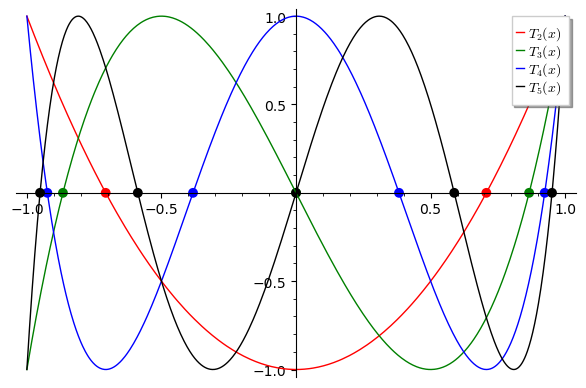
\includegraphics[width=9cm]{img/C1/ceros.png}
        \caption{Polinomios de Tchebichef de tipo I y sus ceros}
        \label{img:ejemplo-ceros}
    \end{figure}

    \newpage

    
\end{ejemplo}

Los ceros de los polinomios ortogonales tienen un papel importante, por ejemplo, en fórmulas de integración numérica, ya que tomar los nodos en los ceros de los polinomios ortogonales reduce considerablemente el error en la integración. Una aplicación bastante directa podrían ser las fórmulas de cuadratura gaussiana (véase \cite[Ch. I, Sección 6]{chihara}). También serán relevantes en los próximos capítulos al jugar $\xi_1$ un papel importante en el soporte de la medida. Incluso tienen una interpretación en el campo del equilibrio electrostático (véase \cite{Steinerberger}).